\documentclass[letterpaper]{article}
\usepackage[submission]{aaai2027}
\usepackage[hyphens]{url}
\usepackage{graphicx}
\urlstyle{rm}
\def\UrlFont{\rm}
\usepackage{natbib}
\usepackage{caption}
\frenchspacing
\usepackage{booktabs}

\pdfinfo{
/TemplateVersion (2027.1)
}

\setcounter{secnumdepth}{0}
\renewcommand{\thefigure}{S\arabic{figure}}
\renewcommand{\thetable}{S\arabic{table}}

\title{Semantic-Geometry Compatibility Learning for Reliable 3D Scene Graph Relations: Supplementary Material}
\author{Anonymous Submission}
\affiliations{}

\begin{document}
\maketitle

\section{Scope and Evaluation Boundary}

This supplement reports validation-level analyses for the scoped H002 claim.
The quantitative route contains higher/lower and bigger/smaller, with a
qualified left/right result reported in the main paper. The figures and tables
below do not establish a hidden-test benchmark, all-family reliability,
support/contact reliability, calibrated selective prediction, or a promoted
learned-geometry score. Violation@K remains a custom geometry-consistency
metric.

\section{Actual Validation-Row Examples}

Figure~\ref{fig:supp-qualitative} visualizes three rows drawn from the frozen
qualitative package. These are row-level examples, not rendered scene images.
They show the two intended operations: filtering a source-high but
geometry-violated edge and promoting a GT-matched, geometry-satisfied edge.

\begin{figure*}[t]
\centering
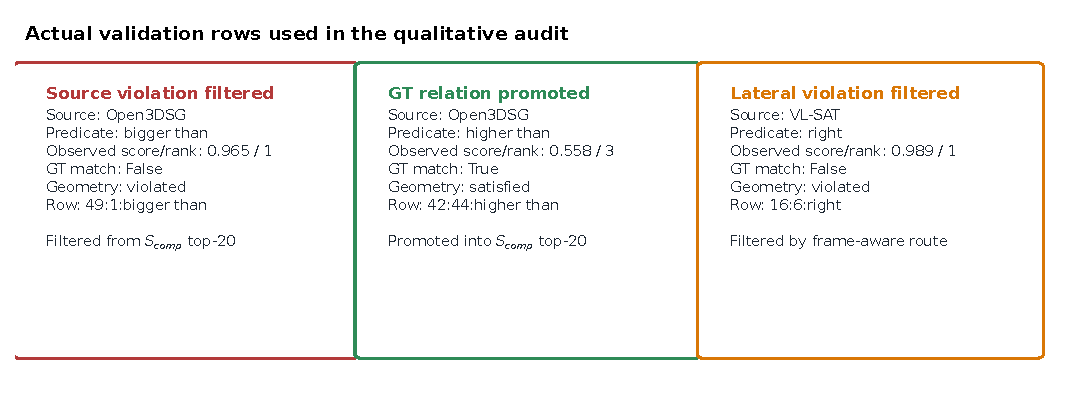
\includegraphics[width=0.98\textwidth]{figures/qualitative_reranking_rows.pdf}
\caption{Actual validation-row examples from VL-SAT and Open3DSG candidate
lists. The examples illustrate reranking behavior and the qualified lateral
route; they are not additional benchmark units or all-family results.}
\label{fig:supp-qualitative}
\end{figure*}

\section{Failure-Route Visualization}

Figure~\ref{fig:supp-failures} separates two failure mechanisms. Front/behind
can reduce the custom violation rate while losing too much recall. The latest
support/contact repair attempt is not an independent reliability target: only
35 of 382 binary rows are positive, the majority baseline is 0.908, and the
geometry-rule construction state recovers the target with 1.0 leave-one-out
accuracy and macro recall. This circularity blocks a metric rerun and any
solved-route claim.

\begin{figure*}[t]
\centering
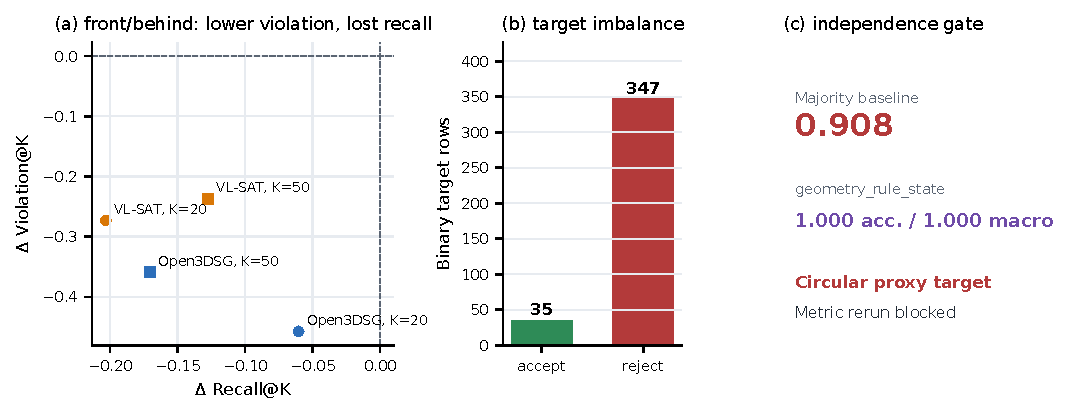
\includegraphics[width=0.98\textwidth]{figures/failure_routes.pdf}
\caption{Failure-route evidence. Left: front/behind reduces Violation@K but
loses recall. Center/right: the support/contact target is sparse and exactly
recoverable from its geometry-rule construction field, so it remains a
diagnostic rather than a reliability result.}
\label{fig:supp-failures}
\end{figure*}

\clearpage
\onecolumn
\section{Full Tables}

\noindent
\begin{minipage}[t]{0.48\textwidth}
\centering
\small
\setlength{\tabcolsep}{4pt}
\begin{tabular}{rcc}
\toprule
K & $\Delta$Recall@K (95\% CI) & $\Delta$Violation@K (95\% CI) \\
\midrule
5 & +0.008 [-0.006, +0.023] & -0.241 [-0.254, -0.228] \\
10 & +0.042 [+0.023, +0.062] & -0.230 [-0.240, -0.220] \\
20 & +0.082 [+0.048, +0.118] & -0.243 [-0.252, -0.235] \\
50 & +0.103 [+0.069, +0.141] & -0.259 [-0.266, -0.252] \\
100 & +0.005 [+0.000, +0.011] & -0.143 [-0.147, -0.139] \\
\bottomrule
\end{tabular}
\captionof{table}{Full validation comparison-route grid for $S_{\mathrm{comp}}-S_{\mathrm{src}}$. The route contains higher/lower and bigger/smaller only; Violation@K is custom and this is not a hidden-test benchmark.}
\label{tab:supp-main-grid}
\end{minipage}
\hfill
\begin{minipage}[t]{0.48\textwidth}
\centering
\small
\setlength{\tabcolsep}{5pt}
\begin{tabular}{lrrr}
\toprule
Variant & K & Main $-$ variant $\Delta$R & $\Delta$V \\
\midrule
Rank percentile & 10 & +0.127 & +0.047 \\
Rank percentile & 20 & +0.084 & +0.027 \\
Rank percentile & 50 & +0.024 & -0.075 \\
Raw product & 10 & +0.015 & +0.001 \\
Raw product & 20 & +0.026 & +0.003 \\
Raw product & 50 & +0.010 & +0.007 \\
\bottomrule
\end{tabular}
\captionof{table}{Normalization sensitivity. Positive $\Delta$R means the frozen min--max score has higher recall; positive $\Delta$V means it has higher violation and is worse on that axis. We do not claim normalization invariance.}
\label{tab:supp-normalization}
\end{minipage}

\vspace{8pt}
\begin{center}
\centering
\small
\setlength{\tabcolsep}{5pt}
\begin{tabular}{lcc}
\toprule
Reference/control at $K=20$ & $\Delta$Recall@20 (95\% CI) & $\Delta$Violation@20 (95\% CI) \\
\midrule
Source score & +0.082 [+0.048, +0.118] & -0.243 [-0.252, -0.235] \\
Geometry-only & +0.078 [+0.047, +0.110] & -0.227 [-0.235, -0.219] \\
Plain concat. & +0.095 [+0.065, +0.131] & -0.230 [-0.239, -0.222] \\
Shuffled $C_e$ & +0.090 [+0.061, +0.118] & -0.278 [-0.288, -0.270] \\
Wrong-$T_e$ & +0.203 [+0.158, +0.249] & -0.585 [-0.602, -0.569] \\
\bottomrule
\end{tabular}
\captionof{table}{Counterfactual and mechanism controls on the validation comparison route. Deltas are $S_{\mathrm{comp}}$ minus the named row. Matched compatibility outperforms source, geometry-only, plain concatenation, shuffled-$C_e$, and wrong-predicate controls.}
\label{tab:supp-controls}
\end{center}

\vspace{5pt}
\begin{center}
\centering
\scriptsize
\setlength{\tabcolsep}{3.5pt}
\begin{tabular}{llrcc}
\toprule
Source & Family & K & $\Delta$Recall@K (95\% CI) & $\Delta$Violation@K (95\% CI) \\
\midrule
Open3DSG & relative vertical & 20 & +0.254 [+0.175, +0.331] & -0.433 [-0.444, -0.423] \\
Open3DSG & relative vertical & 50 & +0.237 [+0.135, +0.329] & -0.324 [-0.337, -0.311] \\
Open3DSG & size relative & 20 & +0.133 [-0.060, +0.362] & -0.371 [-0.382, -0.361] \\
Open3DSG & size relative & 50 & +0.398 [+0.324, +0.470] & -0.341 [-0.354, -0.328] \\
VL-SAT & relative vertical & 20 & +0.003 [-0.006, +0.011] & -0.078 [-0.085, -0.071] \\
VL-SAT & relative vertical & 50 & +0.003 [+0.000, +0.007] & -0.164 [-0.175, -0.154] \\
VL-SAT & size relative & 20 & +0.006 [+0.000, +0.019] & -0.093 [-0.102, -0.085] \\
VL-SAT & size relative & 50 & -0.012 [-0.031, +0.000] & -0.217 [-0.227, -0.207] \\
\bottomrule
\end{tabular}
\captionof{table}{Source/family-wise bootstrap intervals for $S_{\mathrm{comp}}-S_{\mathrm{src}}$. The table exposes heterogeneous cells rather than treating the aggregate as uniform improvement.}
\label{tab:supp-family-ci}
\end{center}

\vspace{5pt}
\begin{center}
\centering
\small
\setlength{\tabcolsep}{5pt}
\begin{tabular}{llll}
\toprule
Audit item & Data & Accuracy/statistic & Balanced statistic \\
\midrule
Target composition & 35 accept / 347 reject & 0.908 majority & -- \\
predicate $\times$ class pair & 382 rows & 0.929 LOO acc. & 0.704 macro recall \\
geometry rule state & 382 rows & 1.000 LOO acc. & 1.000 macro recall \\
geometry core signature & 382 rows & 0.953 LOO acc. & 0.743 macro recall \\
\bottomrule
\end{tabular}
\captionof{table}{Support/contact target-independence audit. Only 35 binary positives remain, the majority baseline is 0.908, and the geometry-rule construction field reconstructs the target with 1.0 leave-one-out accuracy and macro recall. This circularity blocks training, metric reruns, and solved-route wording.}
\label{tab:supp-support-audit}
\end{center}


\end{document}
